%!TEX root = final_report.tex

\section{Algorithm} \label{sec:algorithm}

%%%%%%%%%%%%%%%%%%%%%%
\subsection{Outline}

The classification process is divided in two main phases:

\begin{itemize}
    % \setlength{\itemsep}{8pt}
    \item In the first phase, the material properties are inferred from the images. To achieve this, \emph{SIFT} descriptors are extracted from all the sample images. Next, a vector quantization process is applied over them using \emph{k-means}. The results are finally used as input feature vectors for the \emph{SVMs}, along with manually defined markup of properties.

    \item In the second phase, the material label is obtained using the inferred material properties. For this purpose, the vectors of properties and the real material labels are used as input for \emph{SVMs} and \emph{Naive Bayes} classifiers.
\end{itemize}


%%%%%%%%%%%%%%%%%%%%%%
\subsection{From images to properties}

%%%%%%%%%%%
\subsubsection{Manual markup of properties}

The first step is to manually markup the properties of each of the sample images. This procedure consists on defining its shape and touch for the \emph{fine}, \emph{medium} and \emph{coarse} scales. Figure~\ref{fig:scales} shows an example of the approximate size of them, although its position can be arbitrary.

\begin{figure}[!ht]
    \centering
    \includegraphics[width=0.725\textwidth]{Images/Scales.pdf}
    \caption{Visual representation of the different scales.}
    \label{fig:scales}
\end{figure} 
\FloatBarrier  

The possible values assigned to the three scales for each of the properties are the following:

\begin{itemize}
    \item \textbf{Shape}: \emph{flat}, \emph{round}, \emph{extended organized} or \emph{extended disorganized}.
    \item \textbf{Touch}: \emph{furry}, \emph{feathery}, \emph{coarse}, \emph{bumpy}, \emph{scratchy}, \emph{smooth} or \emph{velvety}.
\end{itemize}

An example of a manually marked image is the following one:

\newcommand{\matName}{Brick}
\newcommand{\imgNumber}{02}
\inputImage{flat}{scratchy}
{extended organized}{coarse}
{extended organized}{coarse}
{}{}

In this case, the material shows a scratchy touch at fine scale, due to the mortar used to join the bricks. At this scale, the shape can be considered flat, since no forms are appreciable. At a medium scale, its touch is mainly coarse, because of the bricks, while some forms extended and organized start to appear. Both properties are the same if the image is considered at a coarse scale. \\

In many cases, several touch or shape properties are available at a given scale in the same sample image. No precedence rules have been defined at this point, which means that any of them is completely valid. 


%%%%%%%%%%%
\subsubsection{Extraction of Scale-Invariant Feature Transform (SIFT) descriptors}

The next step of the\emph{Automatic Material Recognition} algorithm is the extraction of \emph{Scale-Invariant Feature Transform} (\emph{SIFT}) descriptors from each of the sample images. \\

In 2004, David Lowe, from the \emph{University of British Columbia}, came up with this new algorithm in \cite{Lowe_2004_SIFT} to extract keypoints and compute its descriptors from an image. The algorithm involves the following main steps:

\begin{enumerate}
    \item First, potential keypoints are detected. For this, a \emph{Difference of Gaussian} (\emph{DoG}), is convoluted using various values of $\sigma$, which acts as a scaling parameter, with the gray-scale version of the input image. Then, the potential keypoints are obtained finding the local extrema over scale and space in the \emph{DoG}.
    \item Next, once potential keypoints are found, they are filtered to maintain only the interesting ones and increase the accuracy of the results. To achieve this, keypoints containing edges and those without enough intensity are discarded.
    \item Then, an orientation is assigned to each keypoint to achieve invariance to image rotation. For this, the gradient magnitude and direction is calculated in the neighbourhood of each keypoint. 
    \item Finally, keypoint descriptors are created. For this, a 4x4 neighbourhood is takend around the keypoint and a 8 bin orientation histogram is created for each sub-block. This adds up to a total of 128 bin values available, which are represented as a vector to form the keypoint descriptor.
\end{enumerate}

A visual example of the keypoints and descriptors extracted from the material images using \emph{SIFT} algorithm can be seen in figures \ref{fig:Birch10SIFT}, \ref{fig:Brick02SIFT}, \ref{fig:Corduroy05SIFT} and \ref{fig:Feathers11SIFT}.

\plotTwoImages
{Images/50Keypoints1.png}{}{}
{Images/50Descriptors1.png}{}{}
{50 randomly sampled keypoints (on the left) and keypoints with descriptors (on the right) extracted with \emph{SIFT} from \texttt{Birch/10.png}.}{fig:Birch10SIFT}

\plotTwoImages
{Images/50Keypoints2.png}{}{}
{Images/50Descriptors2.png}{}{}
{50 randomly sampled keypoints (on the left) and keypoints with descriptors (on the right) extracted with \emph{SIFT} from \texttt{Brick/02.png}.}{fig:Brick02SIFT}

\plotTwoImages
{Images/AllKeypoints1.png}{}{}
{Images/AllDescriptors1.png}{}{}
{All the keypoints (on the left) and keypoints with descriptors (on the right) extracted with \emph{SIFT} from \texttt{Corduroy/05.png}.}{fig:Corduroy05SIFT}

\plotTwoImages
{Images/AllKeypoints2.png}{}{}
{Images/AllDescriptors2.png}{}{}
{All the keypoints (on the left) and keypoints with descriptors (on the right) extracted with \emph{SIFT} from \texttt{Feathers/11.png}.}{fig:Feathers11SIFT}

Apart from the standard \emph{SIFT} implementation, a dense version of it, called \emph{PHOW}, have been used. The \emph{MATLAB} code where this step is implemented and commented at a low-level can be found in the file \texttt{computeDescriptors.m}.

%%%%%%%%%%%
\newpage
\subsubsection{Vector quantization through \emph{k-means} clustering}

After all the \emph{SIFT} descriptors have been extracted from the material images, a vector quantization process is required, since the raw descriptors cannot be used directly as input features for the \emph{SVMs}. This is due to the variability in the number of descriptors computed for each image. Even if that were not the case, a preprocess step would still be required to convert all the 128-dimensional descriptors of every image into a suitable feature vector. \\

\begin{wrapfigure}{l}{0pt}
    \centering
    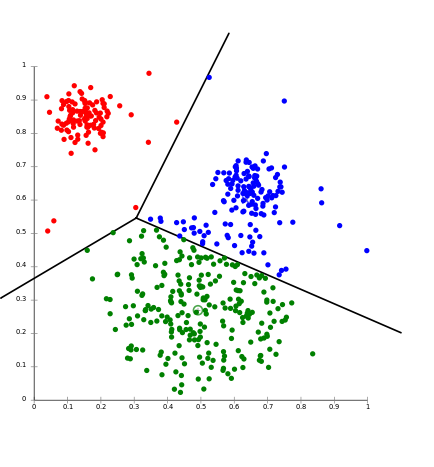
\includegraphics[width=0.45\textwidth, trim=0 30 20 20, clip]
                    {Images/KMeans.png}
    \caption{A visual representation\protect\footnotemark\xspace of the result of \emph{k-means} applied to two-dimensional observations for $k=3$ cluster centers.}
    \label{}
\end{wrapfigure}

\footnotetext{\emph{``KMeans-Gaussian-data"} by Chire - Own work. Licensed under Creative Commons Attribution-Share Alike 3.0 via Wikimedia Commons.}

The vector quantization is based on a \emph{bag-of-words model} to generate the feature vector of each image. First, \emph{k-means} clustering is applied to the extracted \emph{SIFT} descriptors. \\

\emph{K-means} clustering is an algorithm original from signal processing and proposed by Stuart Lloyd in 1982 in its standard version as a technique for \emph{pulse-code modulation} in \cite{Lloyd_1982_LSQ}. It aims to partition \emph{n} observations into \emph{k} clusters in which each observation belongs to the cluster with the nearest mean, serving as a prototype of the cluster. To achieve this, it starts selecting \emph{k} random observations and setting them as cluster centers. Then, it assigns each observation to the closest cluster center and updates the cluster centers by computing the mean of the assigned observations. It repeats the same process till convergence. \\

Therefore, the \emph{SIFT} descriptors are partitioned into \emph{k} clusters, generating \emph{k} clusters centers, which work as \emph{codewords} in the \emph{bag-of-words model}. Finally, each image is assigned a histogram of the \emph{codewords}, which will work as feature vectors in the \emph{SVMs}, by counting the number of \emph{SIFT} descriptors of that image that are ``represented'' by each \emph{codeword}. \\

The \emph{MATLAB} code where this step is implemented and commented at a low-level can be found in the file \texttt{quantizeVectors.m}.

%%%%%%%%%%%
\newpage
\subsubsection{Support Vector Machines (SVMs) for properties recognition}

Once every sample image has its own feature vectors associated, resulting from the vector quantization of the previous step, it is time to train a classifier using them along with the manual markup of properties, which will be the class labels that the classifier will produce. For this purpose, \emph{Support Vector Machines} (\emph{SMVs}) have been used. \\

\begin{wrapfigure}{L}{0pt}
    \centering
    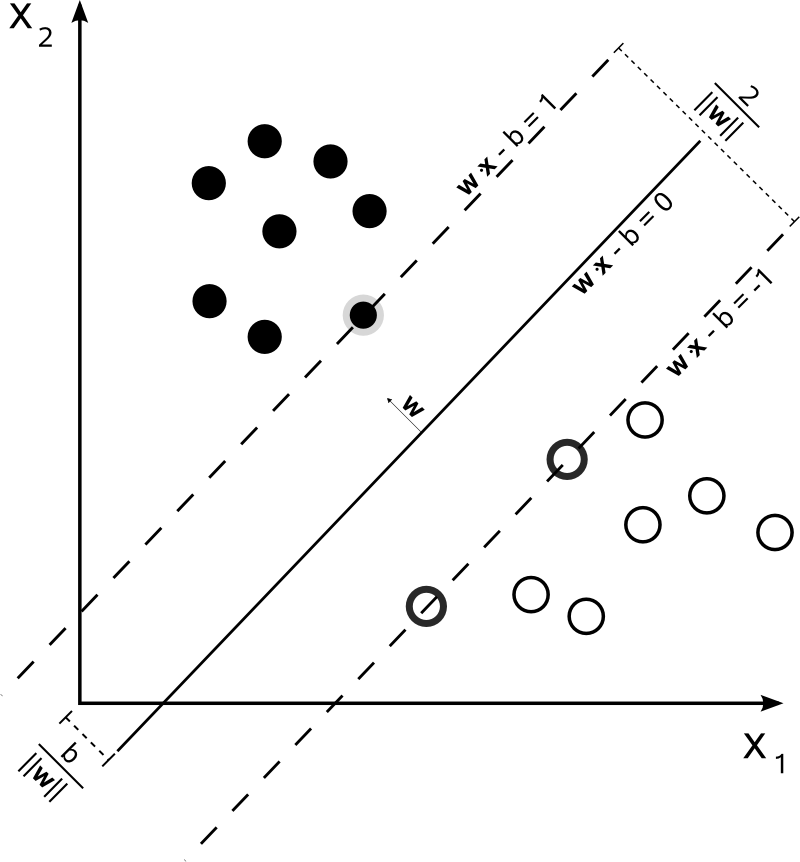
\includegraphics[width=0.4\textwidth, trim=0 0 0 0, clip]
                    {Images/SVMs.png}
    \caption{A visual representation\protect\footnotemark\xspace of the result of the model obtained by a \emph{SVM} algorithm to two-dimensional feature vectors.}
    \label{}
\end{wrapfigure}

\footnotetext{\emph{``Svm max sep hyperplane with margin"} by Cyc - Own work. Licensed under Public domain via Wikimedia Commons.}

\emph{SVMs}, invented by Vladimir Vapnik and published for the first time in \cite{Vapnik_1995_SVMs}, are supervised learning models that work as binary linear classifiers. Given a set of training examples with their respective binary class labels, an \emph{SVM} training algorithm builds a model that assigns, i.e. classifies, new examples into one of the two categories. The built model will define a ($k-1$)-dimensional hyperplane (where \emph{k} is the number of clusters used in the previous step) that will represent the largest separation between the two classes. \\

In our case, one \emph{SVM} is trained for each possible combination of properties and scales that exist in, at least, one of the images of the dataset. In other words, one of the \emph{SVMs} will be used to tell apart material images that present the touch property \emph{bumpy} at \emph{medium} scale, and a different one will decide if a sample is \emph{bumpy} at \emph{coarse} scale, or \emph{extended-organized} at \emph{fine} scale, etc. In the same way, if no image has been manually classified as \emph{feathery} at \emph{fine} scale, no \emph{SVM} will be trained for that property, because of the lack of positive samples. Therefore, the resulting \emph{SVMs}, individually, will only be able to tell if a sample image presents the property at a specific scale or not, since they are binary classifiers. \\

The \emph{MATLAB} code where this step is implemented and commented at a low-level can be found in the file \texttt{svm.m}.


%%%%%%%%%%%%%%%%%%%%%%
\subsection{From properties to materials}

After the properties have been inferred from the material images, a binary feature vector can be built from them for each image considering all the \emph{property-scale} combinations and assigning a 1 if the image has that property or a 0 otherwise.

%%%%%%%%%%%
\subsubsection{Support Vector Machines (SVMs) for material recognition}

The feature vectors combined with the real material labels, allow us to train new \emph{SVMs} for the task of classifying materials from the properties. Unfortunately, the \emph{SVM} model is only suitable for binary classification, i.e., if an image contains a material or not, which is not enough for multi-class classification problem like this. \\

To solve this problem, \emph{Machine Learning} theorists have come up with different strategies. One of them, and the one we use, is \emph{One Vs. All} (\emph{OvA}, a.k.a. \emph{One Vs. Rest} or \emph{OvR}), which consists on training a binary classifier por each class and, when classifying a new sample, applying all of them individually over the sample and considering as result the class of the classifier that gets the highest confidence in the classification. So, for example, if our problem considered three possible materials: \emph{marble}, \emph{brick} and \emph{leather}, and the results of their respective \emph{SVMs} were 3.52, 6.07 and -1.89, the \emph{OvA} would determine that the correct class is \emph{brick}. \\

The \emph{MATLAB} code where this step is implemented and commented at a low-level can be found in the file \texttt{svmOneVsAll.m}.


%%%%%%%%%%%
\subsubsection{Naive Bayes classifier for material recognition}

The properties feature vectors can also be used to fed a different kind of classifier, in this case, more suitable for multi-class classification, as is a \emph{Naive Bayes} classifier. \\

\emph{Naive Bayes} classifiers are another kind of supervised learning models which, unlike \emph{SVMs}, work as probabilistic classifiers instead of linear ones. They are based on the application of the \emph{Bayes' theorem} with strong, i.e. naive, independence assumptions between the features. In other words, it is assummed that the features are independent with respect to each other given the class. \\ 

With all the information computed in the previous steps about the images, a \emph{Naive Bayes} classifier can be trained for material recognition. The \emph{MATLAB} code where this step is implemented and commented at a low-level can be found in the file \texttt{naiveBayes.m}.


